% use KOMAScript
\documentclass{scrartcl}

%--------- font setup --------
% make sure you use XeLaTeX or LuaLaTeX for true Unicode support
% font selection is the matter of choice
\usepackage{fontspec} % font selection
\setromanfont[Numbers=Monospaced]{Linux Libertine O}
\setsansfont[Numbers=Monospaced]{Linux Biolinum O}
% use the fontawesome package if you want fancy symbols
% the Fontawesome font must be installed as well
\usepackage{fontawesome}

%--------- mathematics support (you know you need this!) --------
\usepackage{amsmath,amsthm,amssymb,amsfonts,stmaryrd,mathtools} 

%--------- nicer tables --------
\usepackage{longtable}
\usepackage{ctable, multirow, float}

\setupctable{
  mincapwidth=0.8\textwidth,
  captionskip=0.5em,
  footerwidth
}

\setlength{\tabcolsep}{12pt}

% uncomment to enforce float placement HERE
% \floatplacement{table}{H}


%--------- nicer lists -------
\usepackage{enumitem}

%--------- linguistics support --------
\usepackage{expex}     % glosses, linguistic examples etc

% set up font for linguistic examples
\newfontfamily\glossfont{Gentium Plus Italic}[Scale=MatchLowercase,Ligatures={NoCommon, NoDiscretionary, NoHistoric, NoRequired, NoContextual}]

\newfontfamily\devanagari{Noto Sans Devanagari}[Scale=MatchLowercase,Ligatures={NoCommon, NoDiscretionary, NoHistoric, NoRequired, NoContextual}]


\newfontfamily\japanese{Noto Sans CJK JP}[Scale=MatchLowercase,Ligatures={NoCommon, NoDiscretionary, NoHistoric, NoRequired, NoContextual}]


%--------- various packages --------
\usepackage{graphicx}  % for inclusion of pictures etc.
\usepackage{lipsum} % text fillers

\usepackage{natbib}

%--------- hyperlinks --------
% we set up hyperref to hide the links
% they will work, but the document will look classy
% use hypersetup if you want to have colors
\usepackage[hidelinks]{hyperref}

%--------- clever references --------
\usepackage[capitalise]{cleveref}

%--------- linguistic examples --------
\usepackage{expex}
\lingset{everygla=\glossfont} 

%--------- page setup -------
\KOMAoptions{paper=a4} % set a4 paper
\KOMAoptions{twoside=false} % we want to have one side for the online version
\KOMAoptions{BCOR=15mm} % the binding correction
\KOMAoptions{DIV=13} % how many lines


% make sure the page dimentions are correctly calculated
\recalctypearea 

%--------- title setup -------
\title{My report}
\author{A proper name}
\date{\today}

\begin{document}

\maketitle

\tableofcontents

\section{Introduction}\label{sec:introduction}

Read the manual \citep[to be conviently located under][on the itnernet]{expexguide}! Other interesting stuff mentioned by \citet{kibrik1996godoberi} and \citet{forker2013a-grammar}.


\lipsum[1]

\section{Data}\label{sec:data}

As seen in example \nextx, its an example. 

\ex
I am an example
\xe

\ex
I am another example
\xe

You can see an example in \lastx.

\pex
\a First example

\a Second example

\a Third example
\xe

\ex
\begingl
\gla The cat chases the dog //
\glb ART.DEF cat chase.3.SG ART.DEF dog //
\glb ART N V ART N //
\glft `Die Katze jagt den Hund` //
\endgl
\xe

\ex
\begingl
\gla Mary$_i$ ist sicher, dass es den Hans nicht stören 
würde seiner Freundin ihr$_i$ Herz auszuschütten.//
\glb Mary is sure that it the-acc Hans not annoy would
his-dat girlfriend-dat her-acc heart-acc {out to
throw}//
\glft  ‘Mary is sure that it would not annoy John to reveal her
heart to his girlfriend.’//
\endgl
\xe


\ctable[caption = Example, label=table:example]
{
l% This is the column of ones, left aligned
c% This is the column of twos, middle aligned
r% This is the column of threes, right aligned
}
{}
{
\FL One & Two  & Three \ML
1   & 2    & 3  
\NN
1   & 2    & 3 
\NN
1   & 2    & 4
\LL
}

{\itshape Thisi is italic} and {\bfseries this is bold}.

There is some data in \cref{table:example}. You can also look at \cref{fig:weird}. Refer to \cref{sec:introduction} for more information. Also check out this fancy font for linguistic examples {\glossfont Нехай щастить!}, {\glossfont aàuūę}. We can also do Devanagari, but we need an extra font for this: {\devanagari  देवनागरी }.
Or what about some {\japanese 漢字}? Drop me a \faEnvelopeO\ if you have questions!

\section{Discussion}\label{sec:discussion}

\begin{figure}
    \centering
    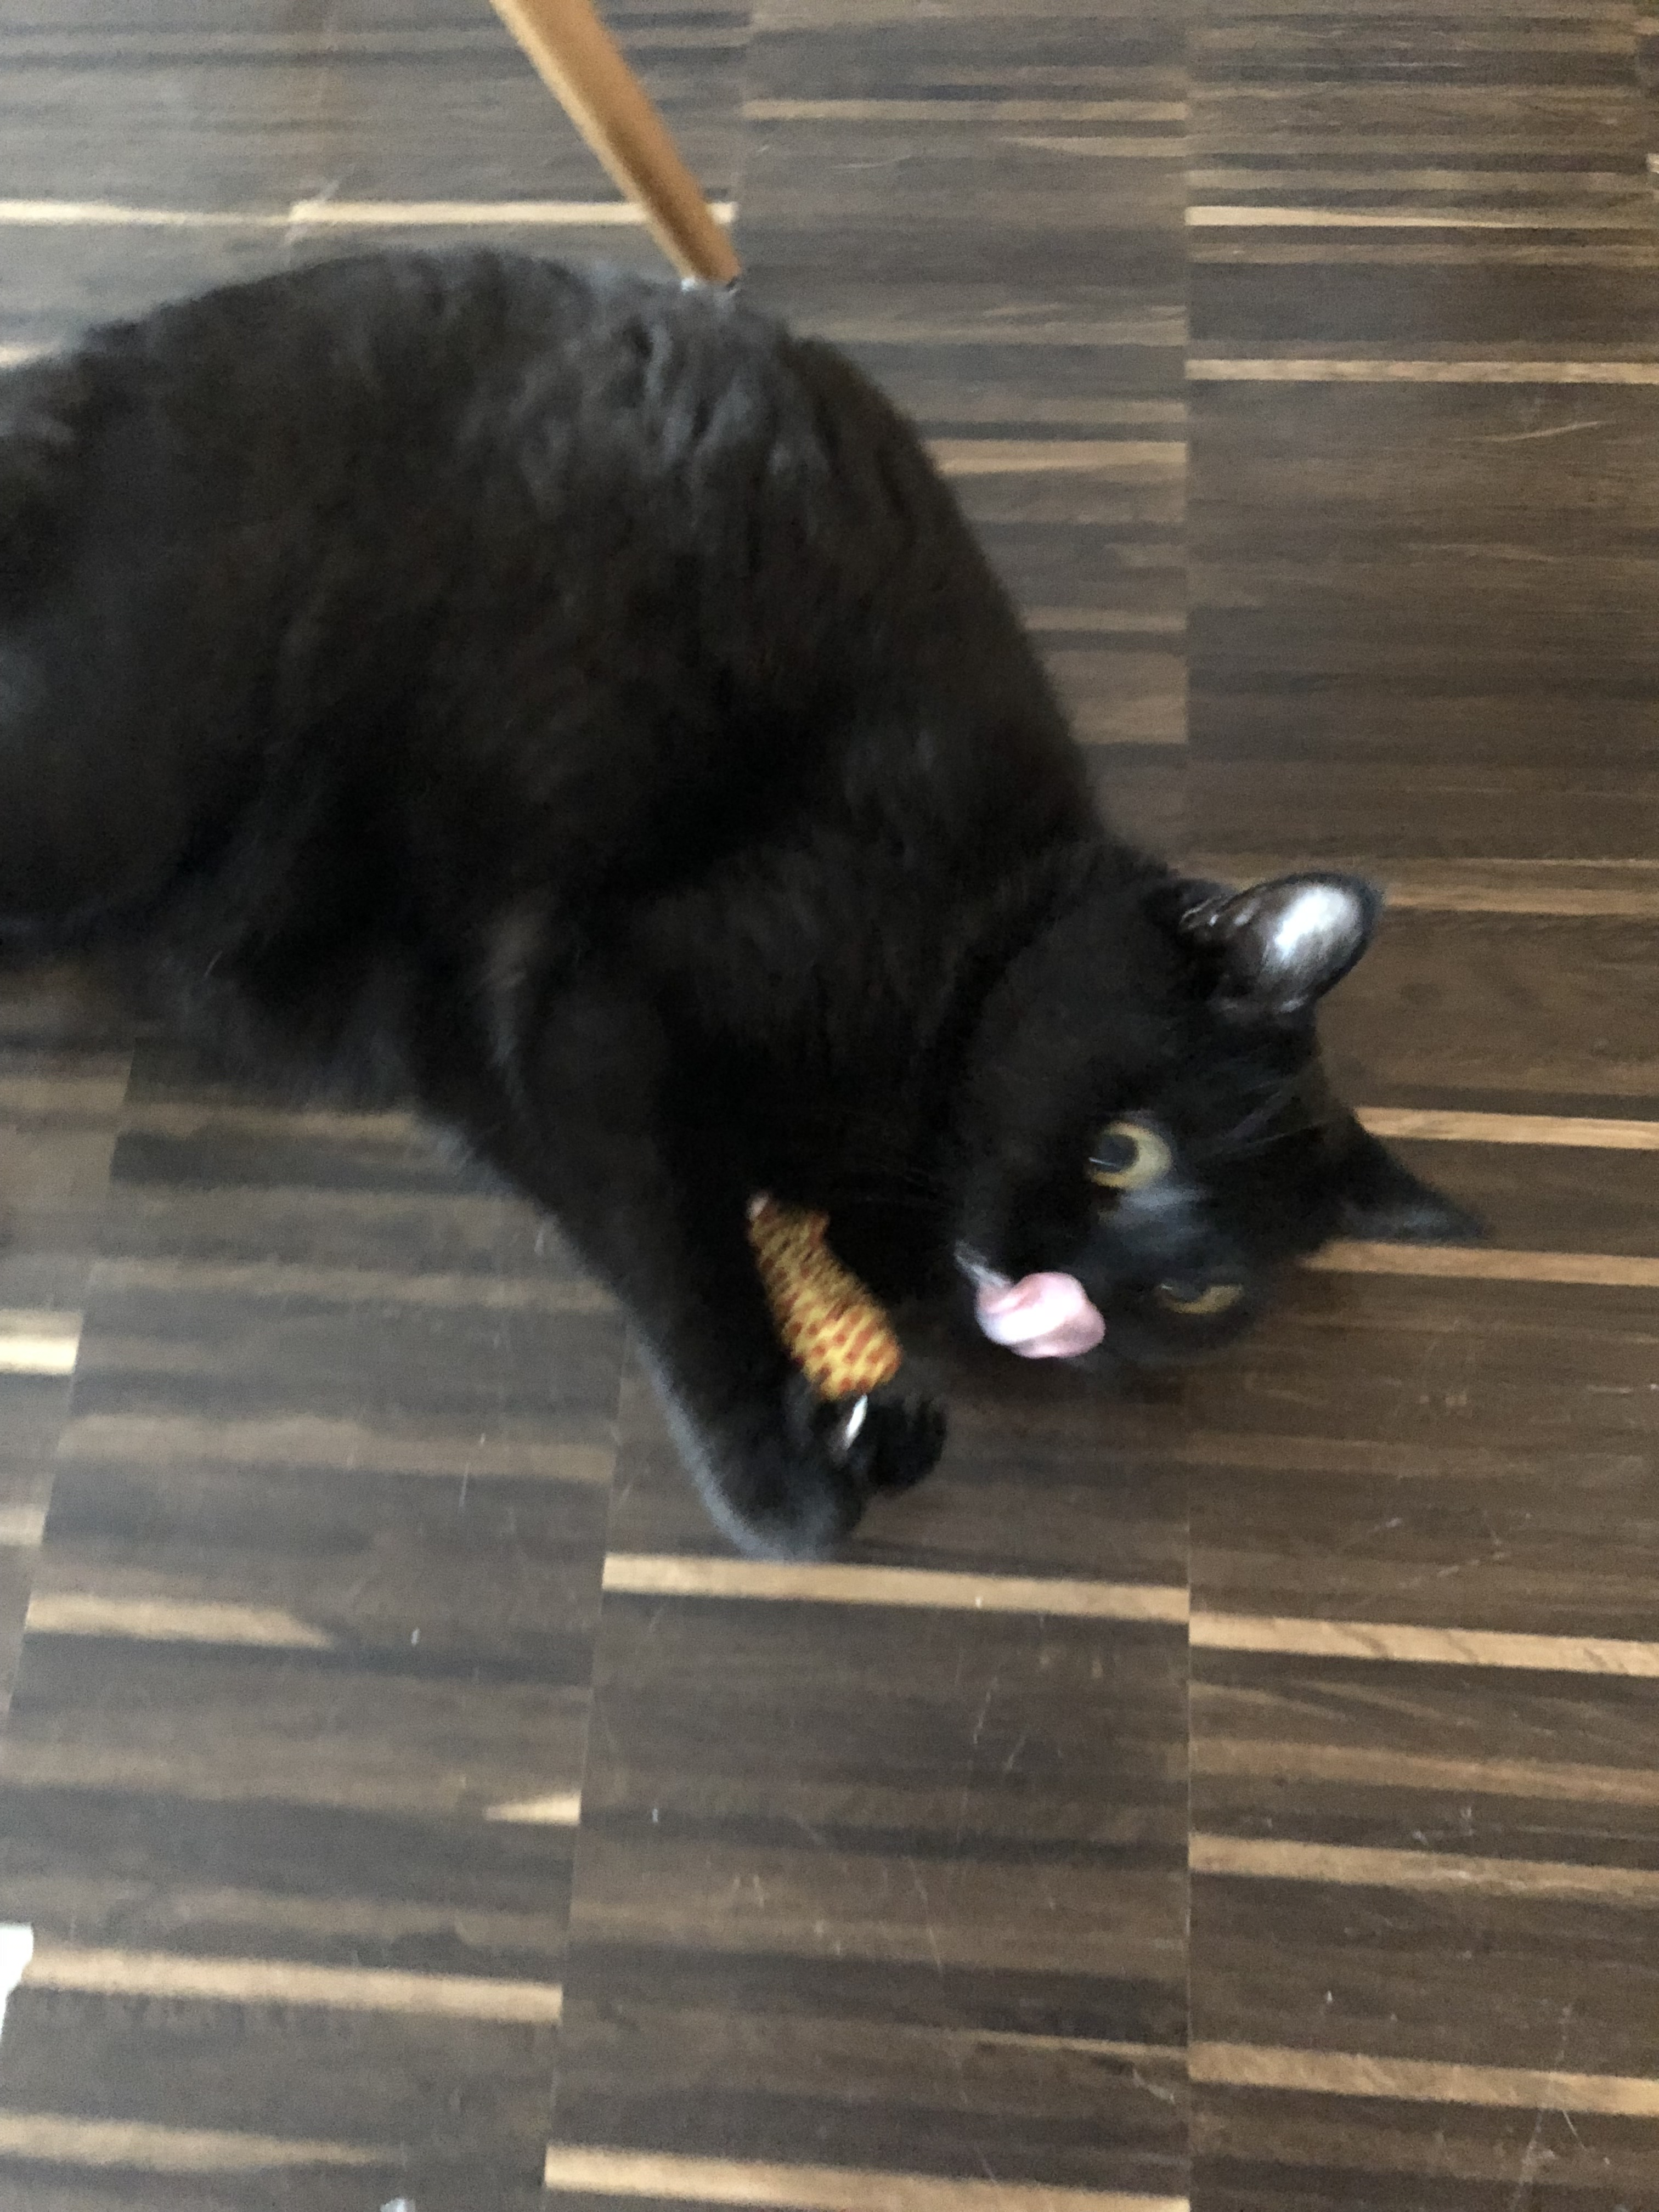
\includegraphics[width=0.7\textwidth]{weird.jpg}
    \caption{Somethign weird}
    \label{fig:weird}
\end{figure}

\lipsum[1]

\section{Conclusion}\label{sec:conclusion}

\lipsum[2]

\bibliographystyle{unified.linguistic}
\bibliography{bibliography}


\end{document}
